
\section{Caching}
Aufgrund der Entscheidung alle Daten verlustfrei im Originalformat zu speichern (\cref{dec:pd:datenspeicherung}), sowie der Verwendung von In-Memory Tabellen-artigen Datenstrukturen, muss sichergestellt werden, dass nicht bei jeder Operation die Originaldaten von Format-Parser neu eingelesen werden müssen.

Aus diesem Grund wurde ein dreistufiges Caching-Konzept für die gesamte Applikation implementiert. Es werden die Caching-Mechanismen von Django mit eingen Modifikationen/Erweiterungen verwendet. Folglich können die Caching-Backends jederzeit durch beliebige von Django unterstützte Backends wie z.B. Memcached, Filesystem, etc. ersetzt werden.
\subsection{Caches}

\cref{fig:pd:caches} zeigt eine Übersicht der in \gls{odh} eingesetzten Caches und deren Storage-Backends.

\begin{figure}[H]
\centering
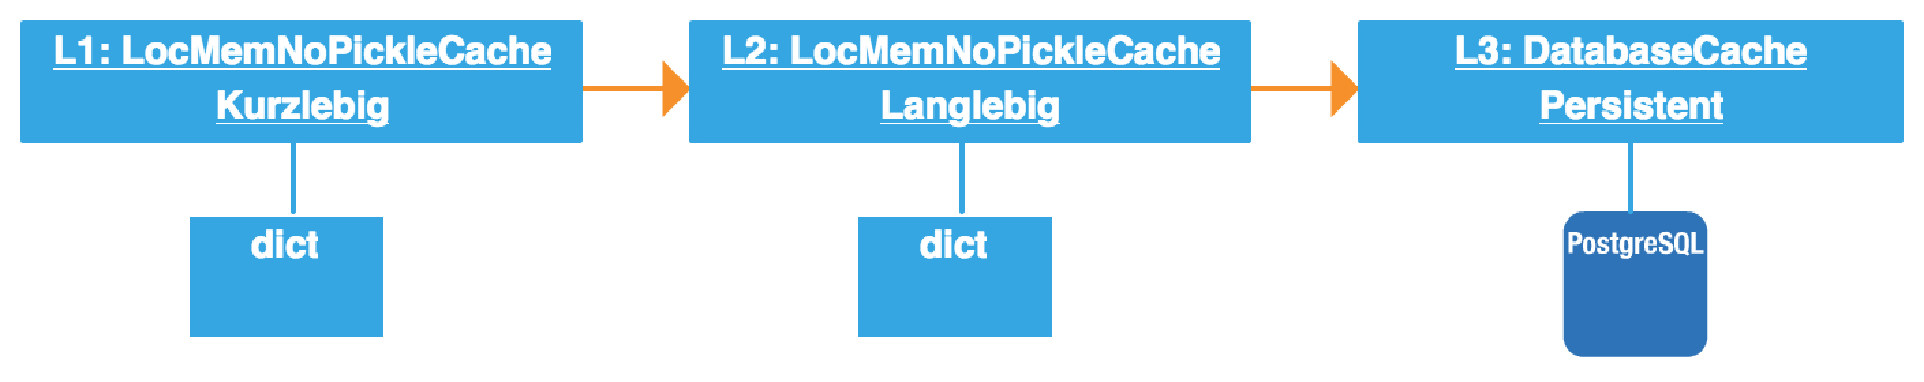
\includegraphics[width=\linewidth]{fig/caching.pdf}
\caption{Übersicht der Caches}
\label{fig:pd:caches}
\end{figure}

\mytable{lX}{
  \textbf{Cache} & \textbf{Beschreibung}\\
  \midrule
  Level 1 & Der Level 1 Cache ist ein In-Memory Cache und sehr kurzlebig (\SI{60}{\second}). Dieser wird hauptsächlich verwendet, um Zwischenresultate wie Format-Konversionen oder Resultate einer Abfrage zu speichern, damit der Benutzer im Webfrontend die Daten sofort mittels Pagination anschauen kann.\\

  Level 2 & Der Level 2 Cache ist ebenfalls ein In-Memory Cache, allerdings werden die Daten länger vorgehalten (\SI{300}{\second}). Darin werden hauptsächlich Daten aus dem Level 3 Cache für mehrere Minuten zwischengespeichert, um Abfrage- und Deserialisierungs-Overhead zu vermeiden.\\

  Level 3 & Der Level 3 Cache ist mit Hilfe eines Datenbank-Backends implementiert. Der Cache speichert eingelesene Dateien im intermediären Format (d.h. DataFrame Objekte) sowie gespeicherte Transformationen ohne Online-Datenquellen.\\
}{Beschreibung der Caches}{pd:caches}

\subsection{Invalidierung}

Überall wo Caching-Mechanismen eingesetzt werden, stellt sich das grosse Problem der Cache-Invalidierung. Wann müssen welche Cache-Einträge invalidiert oder gelöscht werden um falsche oder veraltete Resultate zu verhindern. Da bei \gls{odh} jeweils die DataFrame Objekte von Dateien und Transformationen gespeichert werden, muss wie folgt invalidiert werden:

\begin{itemize}
	\item sobald die Daten einer Online-Quelle\footnote{Beispielsweise ein \acs{wfs} Webservice} sich ändern bzw. neu Angefordert wurden,
	\item wenn eine Transformation modifiziert wird, welche von anderen Transformationen verwendet wird (rekursiv),
	\item oder sobald Daten gelöscht werden.
\end{itemize}

Hierfür wird eine Zwischentabelle in der Datenbank benötigt, um festzuhalten, welche Transformation/Daten von welchen Transformationen referenziert werden. Diese Information wird dann zugleich für die Navigation zwischen Daten und Transformationen im Frontend wiederverwendet\footnote{Welche Daten/Transformationen haben assoziierte Transformationen}. Um jeweils alle zu einem Cache-Key\footnote{Ursprünglich ein Tupel, z.B. \path{('TRF', 10, `CSV')}} gehörenden Einträge zu löschen, wurden die eingebauten Django-Caches so erweitert, dass für alle verwendeten Caching-Provider\footnote{In-Memory und Datenbank} ein kaskadierendes Löschen möglich ist. So lassen sich beispielsweise durch das Löschen von \path{('TRF', 12)} alle gespeicherten und konvertierten Daten, die zu der Transformation mit der ID 12 gehören, ``kaskadierend'' löschen\footnote{Also auch \path{('TRF', 12, `KML')} etc.}
